%!TEX root = ../../main.tex

Her vises overordnede sekvensdiagrammer for hver use case, til at give et overblik over systemets funktionalitet, så det gerne skulle blive lettere at forstå systemmet, og dets interaktion med aktører. Dette skulle gerne vise et bedre indblik på de forskellige interaktioner for den ydre verden. 

\subsection{Overordnede sekvensdiagram for use case 1 - aflæse målinger}
Diagrammet viser interaktion mellem system og bruger for use case 1 - aflæse målinger.

\begin{figure}[H]
    \centering
    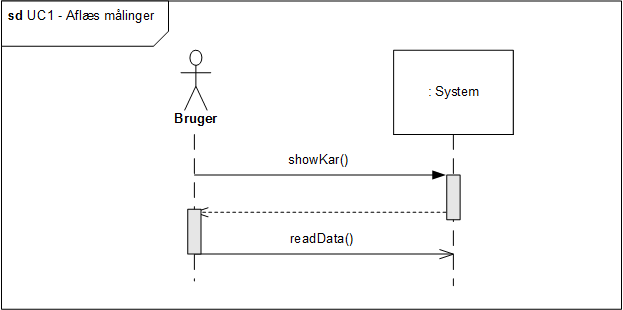
\includegraphics[width=0.8\textwidth]{Systemarkitektur/OverordnedeSekvensdiagrammer/sd_UC1.PNG}
    \caption{sd - use case 1}
    \label{fig:sd_UC1}
\end{figure}

\subsection{Overordnede sekvensdiagram for use case 2 - manuel vanding}
Diagrammer viser interaktion mellem system og bruger for use case 2 - manuel vanding.

\begin{figure}[H]
    \centering
    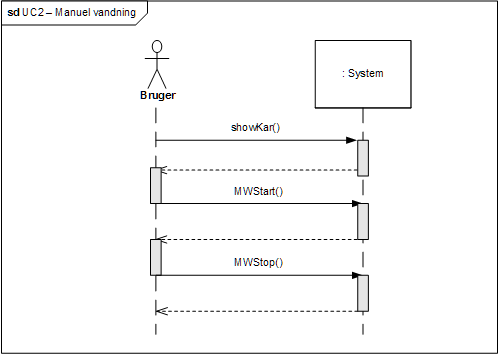
\includegraphics[width=0.8\textwidth]{Systemarkitektur/OverordnedeSekvensdiagrammer/sd_UC2.PNG}
    \caption{sd - use case 2}
    \label{fig:sd_UC2}
\end{figure}


\subsection{Overordnede sekvensdiagram for use case 3 - Indtast pH-værdien}
Diagrammer viser interaktion mellem system og bruger for use case 3 - Indtast pH-værdien.

\begin{figure}[H]
    \centering
    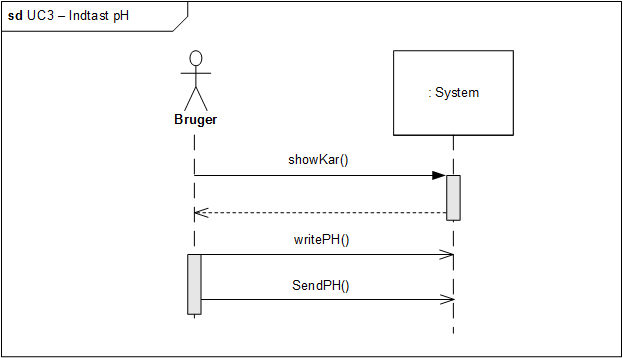
\includegraphics[width=0.8\textwidth]{Systemarkitektur/OverordnedeSekvensdiagrammer/sd_UC3.PNG}
    \caption{sd - use case 3}
    \label{fig:sd_UC3}
\end{figure}

\subsection{Overordnede sekvensdiagram for use case 4 - Indtast pH-værdien}
Diagrammer viser interaktion mellem system og bruger for use case 4 - Indtast volumen.

\begin{figure}[H]
    \centering
    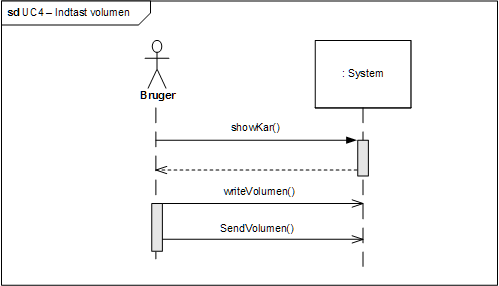
\includegraphics[width=0.8\textwidth]{Systemarkitektur/OverordnedeSekvensdiagrammer/sd_UC4.PNG}
    \caption{sd - use case 4}
    \label{fig:sd_UC4}
\end{figure}

\subsection{Overordnede sekvensdiagram for use case 5 - Indtast pH-værdien}
Diagrammer viser interaktion mellem system og bruger for use case 5 - Opret kar.

\begin{figure}[H]
    \centering
    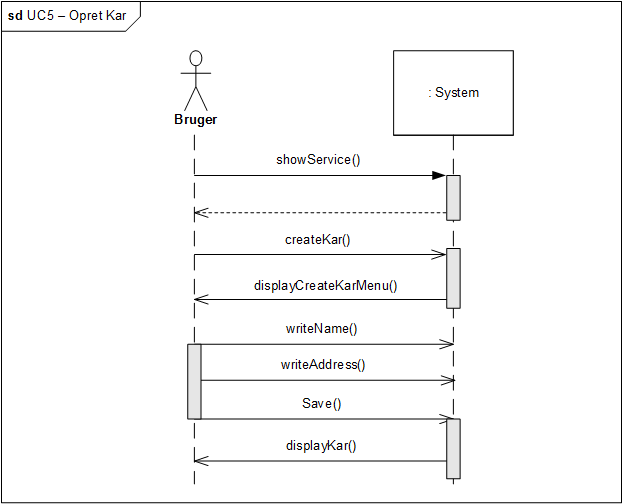
\includegraphics[width=0.8\textwidth]{Systemarkitektur/OverordnedeSekvensdiagrammer/sd_UC5.PNG}
    \caption{sd - use case 5}
    \label{fig:sd_UC5}
\end{figure}

\subsection{Overordnede sekvensdiagram for use case 6 - Indtast pH-værdien}
Diagrammer viser interaktion mellem system og bruger for use case 6 - Slet kar.

\begin{figure}[H]
    \centering
    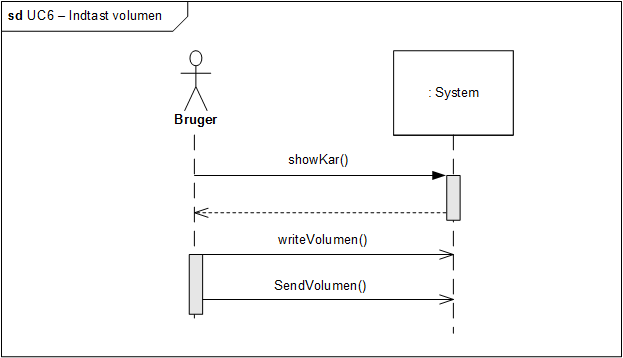
\includegraphics[width=0.8\textwidth]{Systemarkitektur/OverordnedeSekvensdiagrammer/sd_UC6.PNG}
    \caption{sd - use case 6}
    \label{fig:sd_UC6}
\end{figure}